%% Standard-Vorspann
\documentclass[a4paper,11pt,oneside]{article}
\usepackage{ngerman}                   
\usepackage[utf8]{inputenc}
\usepackage[T1]{fontenc}
\usepackage[fleqn]{amsmath}

%% Auf Schriftart Palatino umschalten
\usepackage{mathpazo}
\usepackage[scaled=.95]{helvet}
\usepackage{courier}

%% fast immer benoetigte Pakete
\usepackage{epsfig}
\usepackage{amssymb}
\usepackage{alltt}
\usepackage{latexsym}
\usepackage{makeidx}
\usepackage{textcomp}
\usepackage{rotating}
\usepackage{color}
\usepackage{caption}
\usepackage{verbatim}
\usepackage{fancyhdr}

%packages for codelisting see: http://stackoverflow.com/questions/741985
\usepackage{color, xcolor}
\usepackage{listings}
\usepackage{courier}

\usepackage[
  plainpages=false,
  unicode=true,          % non-Latin characters in Acrobat?s bookmarks
  pdftitle=,
  pdfauthor=GSM OpenBTS Handover Action Group,
  pdftoolbar=true,        % show Acrobat?s toolbar?
  pdfmenubar=true,        % show Acrobat?s menu?
  pdffitwindow=true,     % window fit to page when opened
  pdfstartview={FitV},    % fits the width of the page to the window
  pdfnewwindow=true,      % links in new window
  colorlinks=true,       % false: boxed links; true: colored links
  linkcolor=red,          % color of internal links
  citecolor=green,        % color of links to bibliography
  filecolor=magenta,      % color of file links
  urlcolor=cyan,          % color of external links
  hyperfootnotes=false,
  bookmarks,
]{hyperref}

%Konfigutation für Codelisting
%see: http://stackoverflow.com/questions/741985
\lstset{
	basicstyle=\footnotesize\ttfamily, % Standardschrift
	numbers=left,               % Ort der Zeilennummern
	numberstyle=\tiny,          % Stil der Zeilennummern
	numbersep=5pt,              % Abstand der Nummern zum Text
	tabsize=2,                  % Groesse von Tabs
	extendedchars=true,         %
	breaklines=true,            % Zeilen werden Umgebrochen
	stringstyle=\ttfamily, % Farbe der String
	showspaces=false,           % Leerzeichen anzeigen ?
	showtabs=false,             % Tabs anzeigen ?
	xleftmargin= 17pt,
	framexleftmargin=17pt,
	framexrightmargin=5pt,
	framexbottommargin=4pt,
	showstringspaces=false      % Leerzeichen in Strings anzeigen ?        
}
\lstloadlanguages{PHP, XML, HTML}
\DeclareCaptionFont{white}{\color{white}}
\DeclareCaptionFormat{listing}{\colorbox[cmyk]{0.43, 0.35, 0.35,0.01}{\parbox{\textwidth}{\hspace{15pt}#1#2#3}}}
\captionsetup[lstlisting]{format=listing,labelfont=white,textfont=white, singlelinecheck=false, margin=0pt, font={bf,footnotesize}}

\newcommand{\utsection}[2]{%Section mit Untertitel (ut)
    \section[#1]{#1\newline\normalfont\small\textit{Von: #2}}
}
\newcommand{\utsubsection}[2]{%Subsection mit Untertitel (ut)
    \subsection[#1]{#1\newline\normalfont\small\textit{Von: #2}}
}	
		
%% spezielles Zeug
\usepackage{Abschlussarbeit}

%% Index erzeugen
\makeindex

%% jetzt geht's los
\begin{document}
\raggedbottom


% Vorspann der Arbeit
%
\begin{titlepage}
\begin{flushright}
\includegraphics[width=70mm]{img/hm}%
\end{flushright}

\vspace*{20mm}
\begin{center}
{\Large Hochschule München}\\
{\large Fakultät für Mathematik und Informatik}\\

\vspace*{15mm}
{\huge Projektdokumentation Mobile Netze}\\

\vspace*{10mm}
{\huge \bfseries{Handover mit OpenBSC und OpenBTS}} \\
\vspace*{15mm} 
\end{center}

\vspace*{30mm}

\begin{tabular}{lll}
\textbf{\large {Autoren:}} & & \large {Max Eschenbacher, B.Eng.}\\
			   & & \large {Stefan Giggenbach, B.Eng.}\\
			   & & \large {Thomas Waldecker, B.Eng.}\\
& & \\

\textbf{\large {Abgabe:}} & & \large {19.03.2012}\\
& & \\

\textbf{\large {betreut von:}} & & \large {Prof. Dr. Alf Zugenmaier}\\
& & \\
\end{tabular}

\end{titlepage}

%% Inhaltsverzeichnis
\tableofcontents
\newpage
  
\utsection{Einleitung}{Stefan Giggenbach}

Im Rahmen des Moduls Mobile Netze im Masterstudiengang Informatik wird mit der Durchfürhung einer Projektarbeit, dass in der Vorlesung vermittelte Wissen vertieft und um praktische Aspekte ergänzt. In der vorliegenden Projektarbeit wurde die Handover-Funktionalität in einem GSM-Netzwerk untersucht. In diesem Kapitel wird nach einer theoretischen Einführung in die GSM-Handover-Thematik das Projektziel und die entsprechende Vorgehensweise beschrieben.

\subsection{GSM-Handover}\label{sec:handover}

Der Handover stellt in einem GSM-Netzwerk eine wichtige Aufgabe des Mobility Management dar. Ändert ein Teilnehmen bei aktiver Verbindung seinen Standort, ist es möglich das er den von einer Funkzelle abgedeckten Bereich verlässt. In einem solchen Fall wird die Verbindung durch den Wechsel (Handover) zu einer angrenzenden Nachbarzelle aufrecht erhalten. Grundsätzlich unterscheidet man in einem GSM-Netzwerk folgende Handoverszenarien \cite{bib:grundkursmks}:

\begin{itemize}
 \item Intra BSC Handover
 \item Inter BSC Handover
 \item Inter MSC Handover
 \item Subsequent MSC Handover
\end{itemize}

Die Unterschiede in den Abläufen der einzelnen Szenarien werden in \cite{bib:grundkursmks} ausführlich beschrieben. Aus Sicht der Mobile Station unterscheiden sich die genannten Handoverszenarien nicht. Im folgenden werden nur die Abläufe des Intra BSC Handover beschrieben, die für das Verstädnis der Arbeit entscheidend sind.

Während einer aktiven Verbindung wird der BSC in regelmäßigen Zeitäbständen über die Signalqualität im Up- bzw. Downstream informiert. Zu diesem Zweck sendet die Mobile Station über den SACCH sogenannte Measurement Reports, die anschließend im BSC zur Bestimmung der Downstream-Signalqualität ausgewertet werden. In den Measurement Reports sind neben Messergebnissen zur aktuell verwendeten BTS auch Messergebnisse zu benachbarten BTS, die auf Anweisung des BSC während den Sendepausen von der Mobile Station ermittelt werden. Die Signalqualität des Upstreams wird durch Messergebnisse aus der entsprechenden BTS ebenfalls im BSC berechnet. Der BSC kann aufgrund der eingehenden Measurement Reports zu dem Ergebnis kommen, dass ein Handover zwischen zwei benachbarten BTS notwendig ist, um einen Abbruch der Verbindung zu verhindern.

\begin{figure}[h!]
  \centering
  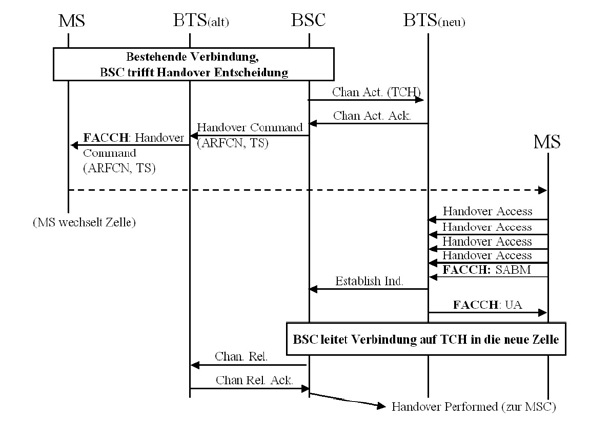
\includegraphics[width=0.85\textwidth]{img/handover.png}
  \caption{Ablaufdiagramm eines Handover \cite{bib:grundkursmks}}
  \label{fig:adhandover}
\end{figure}

Abbildung \ref{fig:adhandover} zeigt den Ablauf eines Handover nach der Entscheidung eines BSC. Im ersten Schritt wird ein TCH in der neuen BTS aufgebaut. War dieser Vorgang erfolgreich, wird der Mobile Station über den FACCH der bestehenden Verbindung ein Handover Command übermittelt. Das Handover Command enthält als wichtige Parameter die Frequenz und den Timeslot des TCH der neuen BTS. Nach der Synchronisation der Mobile Station mit der neuen BTS, sendet es in vier aufeinanderfolgenden Bursts eine Handover Access Message und anschließend eine Set Asynchronous Balanced Mode Message. Die neue BTS quittiert den erfolgreichen Handover mit einem Established Indicator gegenüber dem BSC und einer UA Massage gegenüber der Mobile Station. Nachdem der BSC die Verbindung auf den neuen TCH umschaltet, wird der TCH in der alten BTS abgebaut. Der Handover Vorgang ist damit abgeschlossen.

Die wichtigesten Punkte für die Analyse bzw. Impelmentierung einer Handover-Funktionalität sind damit:

\begin{itemize}
 \item Erfassung und Auswertung der Measurement Reports
 \item Logik für die Entscheidungsfindung eines Handover
 \item Inter BTS Kommunikation zum Aufbau neuer TCH
 \item Erzeugen und Senden eines Handover Command
 \item Umschalten der bestehenden Verbindung und Abbau des alten TCH
\end{itemize}

\subsection{Projektziel und -durchführung}

Ziel der Projektarbeit ist die Integration der in Abschnitt \ref{sec:handover} eingeführten Handover-Funktionalität in die Opensource Software OpenBTS. Das OpenBTS Projekt ermöglicht, zusammen mit einer entsprechenden Radio-Hardware und zusätzlichen Software-Komponenten (GNURadio und Asterisk), den Betrieb eines kompletten GSM-Netzwerks. Mit der kommerziell vertriebenen Version der Software ist bereits ein Handover zwischen zwei BTS möglich. Die Vorraussetzungen für eine erfolgreiche Integration eines Handover-Moduls sind somit gegeben. Die Architektur und Inbetriebnahme des verwendeten OpenBTS-Systems werden in Kapitel \ref{sec:openbts} ausführlich behandelt.

Vor der Integrations- und Implementierungsphase wird der Ablauf eines Handover genauer analysiert. Zu diesem Zweck wird ein OpenBSC-System aufgesetzt, mit dem das in Abschnitt \ref{sec:handover} beschriebene Handoverszenario reproduziert werden kann. Der Aufbau, die Inbetriebnahme und die Konfiguration des OpenBSC-Systems für die Durchführung eines Intra BSC Handover wird in Kapitel \ref{sec:openbsc} behandelt. Die anschlißende Analyse der durchgeführten Handover erfolgt mit Hilfe der auf der Um- und Abis-Schnittstelle erstellen Wireshark Traces und ist in Abschnitt \ref{sec:analyse} beschrieben.

Der Architekturentwurf für die Integration und die teilweise durchgeführte Implementierung des Handover-Moduls werden in Kapitel \ref{sec:hom} behandelt. Der erreichte Projektstand und geschaffene Ansatzpunkte für weitere Projektarbeiten an der Integration des Handover-Moduls schließen die Arbeit ab.



%\include{kap1}
\utsection{OpenBSC}{Stefan Giggenbach}\label{sec:openbsc}

\subsection{Überblick}

Bei OpenBSC handelt es sich wie bei OpenBTS um ein Open Source Projekt. Die Entwicklung erfolgt vollständig in der Sprache C und hat keinen direkten Bezug zum OpenBTS Projekt. Der große Vorteil von OpenBSC liegt in der \textit{network in the box} (nitb) genannten Version, die ohne zusätzliche Software-Komponenten den Betrieb eines GSM-Netzwerks ermöglicht. Mit OpenBSC wird zu einem sehr frühen Zeitpunkt im Projekt ein GSM-Netzwerk mit Handover-Funktionalität betrieben mit dem die entsprechenden Abläufe analysiert werden können (siehe Kapitel \ref{sec:analyse}).

\begin{figure}[h!]
  \centering
  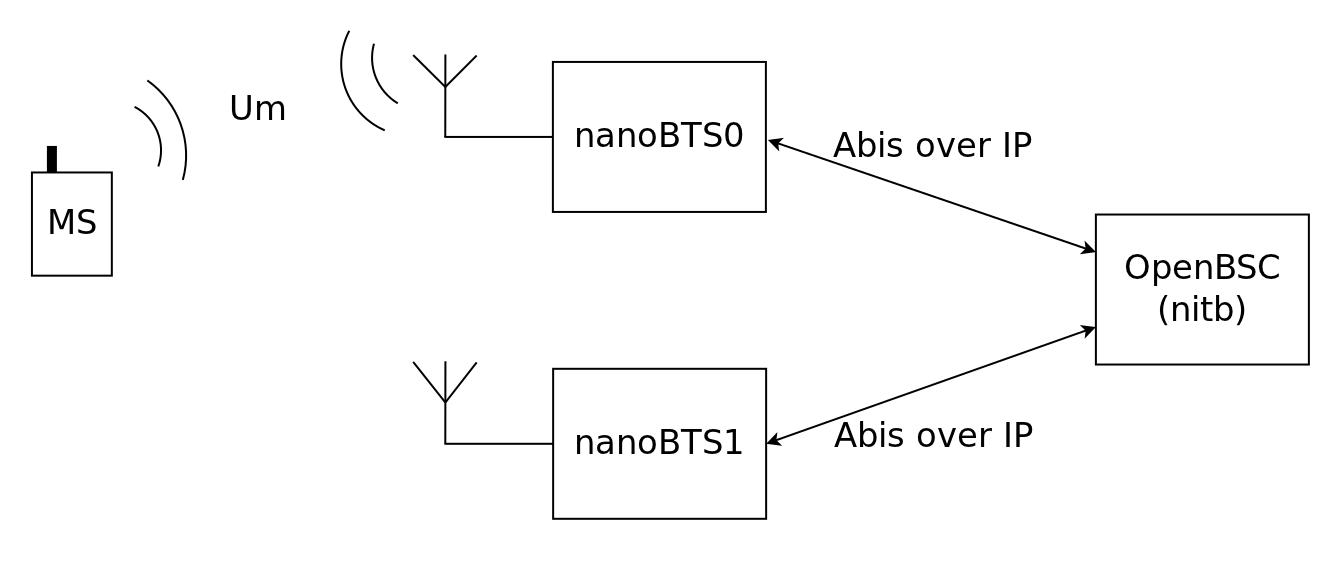
\includegraphics[width=0.9\textwidth]{img/openbscarch}
  \caption{OpenBSC Versuchsaufbau}
  \label{fig:openbscarch}
\end{figure}

Abbildung \ref{fig:openbscarch} zeigt den im Projekt verwendeten Versuchsaufbau. OpenBSC übernimmt nicht nur die Aufgaben des BSC, sondern auch die des MSC. Die Teilnehmerdatenbanken HLR und VLR werden mit einer SQLite3 Datenbank realisiert. Wie in Abbildung \ref{fig:openbscarch} dargestellt, werden zwei nanoBTS der Firma ip.access verwendet. Diese werden über getrennte Abis-over-IP-Schnittstellen an OpenBSC angebunden. Mit dem dargestellten Versuchsaufbau ist somit die Durchführung eines in Abschnitt \ref{sec:handover} beschriebenen Intra BSC Handover mit verhältnismäßig geringem Installations- und Konfigurationsaufwand möglich.

\subsection{Installation und Konfiguration}

Die Installation von OpenBSC ist ausführlich im Wiki des Projekts \cite{bib:buildopenbsc} dokumentiert. In diesem Abschnitt werden nur die wichtigsten Punkte der Installation und die Konfiguration des Systems für den Multi-BTS-Betrieb behandelt.

OpenBSC (nitb) besteht aus insgesamt drei Komponenten:

\begin{itemize}
 \item \textit{libosmocore} - Die Kernbibliothek, die auch für andere Projekte (z.\,B. OsmoBTS) verwendet wird.
 \item \textit{libosmo-abis} - Die Bibliothek zur Umsetzung der Abis- und Abis-over-IP-Schnittstellen.
 \item \textit{openbsc} - Die eigentliche OpenBSC-Software, welche auch die nitb Version enthält.
\end{itemize}

Nach der Kompilierung und Installation dieser drei Komponenten können die beiden nanoBTS, die sich im selben IP-Netzwerk befinden müssen, konfiguriert werden. Dazu werden die zwei Anwendungen \lstinline{./ipaccess-find} und \lstinline{./ipaccess-config} im Verzeichnis \lstinline{<openbsc>/src/ipaccess} benötigt. Die Verwendung der beiden Anwendungen und die benötigten Parameter zur Konfiguration werden ebenfalls im Wiki des Projekts \cite{bib:ipaccess} erläutert. Die bei der Konfiguration der nanoBTS vergebene UnitID wird dabei für die im Folgenden beschriebene Konfiguration von OpenBSC benötigt.

Um den Betrieb beider nanoBTS und die Handover-Funktionalität von OpenBSC zu aktivieren, muss die Konfigurationsdatei von OpenBSC modifiziert werden. Als Grundlage wird die Beispielkonfiguration \lstinline{<openbsc>/doc/examples/osmo-nitb/nanobts/openbsc.cfg} verwendet. Listing \ref{lst:config} zeigt auszugsweise die wichtigsten Inhalte der modifizierte Konfigurationsdatei.

\begin{lstlisting}[label=lst:config,caption=OpenBSC Konfigurationsdatei (Auszug)]
!
! OpenBSC (0.10.1.40-2935) configuration saved from vty
.
network
 network country code 262
 mobile network code 98
 .
 handover 1
 .
 bts 0
  type nanobts
  band DCS1800
  cell_identity 0
  .
  ip.access unit_id 42 0
  .
  trx 0
   rf_locked 0
   arfcn 846
   nominal power 23
   max_power_red 22
   .
 bts 1
  type nanobts
  band DCS1800
  cell_identity 1
  .
  ip.access unit_id 43 0
  .
  trx 0
   rf_locked 0
   arfcn 867
   nominal power 23
   max_power_red 22
   .
\end{lstlisting}

Neben dem Network Country Code und dem Mobile Network Code (Zeilen 5 und 6) muss in den Netzwerkeinstellungen die Handover-Funktionalität gesetzt werden (Zeile 8). Die Konfiguration der beiden nanoBTS beschränkt sich im Wesentlichen auf die Vergabe der eindeutigen CellIDs (Zeilen 13 und 26), der vorher festgelegten UnitIDs (Zeilen 15 und 28) und den beiden Frequenzen (ARFCN in Zeilen 19 und 32).

Nach der Modifikation der Konfigurationsdatei wird diese im Verzeichnis \lstinline{<openbsc>/src/osmo-nitb} gespeichert. Anschließend kann das System mit dem Befehl \lstinline{./openbsc} im selben Verzeichnis gestartet werden. Die Bedienung von OpenBSC erfolgt nach dem Start über eine Telnetsitzung auf Port 4242. Mit Hilfe des Command Line Interfaces der Telnetsitzung ist auch die Administration der Teilnehmerdatenbank möglich. Die Verwendung des CLI ist aufgrund der interaktiven Eingabe selbsterklärend.

Um einen Handover auszulösen, kann bei aktiver Verbindung entweder die Position einer Mobile Station verändert werden oder die Signalqualität wird durch entsprechende Schirmung der Geräte in ausreichendem Umfang reduziert. Die Analyse der mit OpenBSC durchgeführten Handover wird in Kapitel \ref{sec:analyse} detailliert beschrieben.

\utsubsection{Analyse}{Thomas Waldecker}



\utsection{OpenBTS}{Max Eschenbacher}



\subsection{Überblick}



\subsection{Architektur}



\subsection{Inbetriebnahme}



\section{Erweiterungen OpenBTS}



\subsection{Measurement Reports}



\utsubsection{Handover-Modul}{Stefan Giggenbach}\label{sec:hom}

Das implementierte Handover-Modul muss im Prinzip die am Ende des Abschnitts \ref{sec:handover} beschriebenen Aufgaben abarbeiten. Die Erfassung der Measurement Reports wurde bereits in Abschnitt \ref{sec:measrep} beschrieben. Dabei wird, wie bereits erwähnt, nicht die vorhandene SQLite3-Datenbank, sondern zwei neu erstellte Klassen, deren Klassendiagramme in Abbildung \ref{fig:homclass} dargestellt sind, verwendet. Die Definition und Implementierung befindet sich in den Dateien \lstinline{GSMHandover.h} und \lstinline{GSMHandover.cpp} des \textit{GSM}-Moduls.

\begin{figure}[h!t!b!p!]
  \centering
  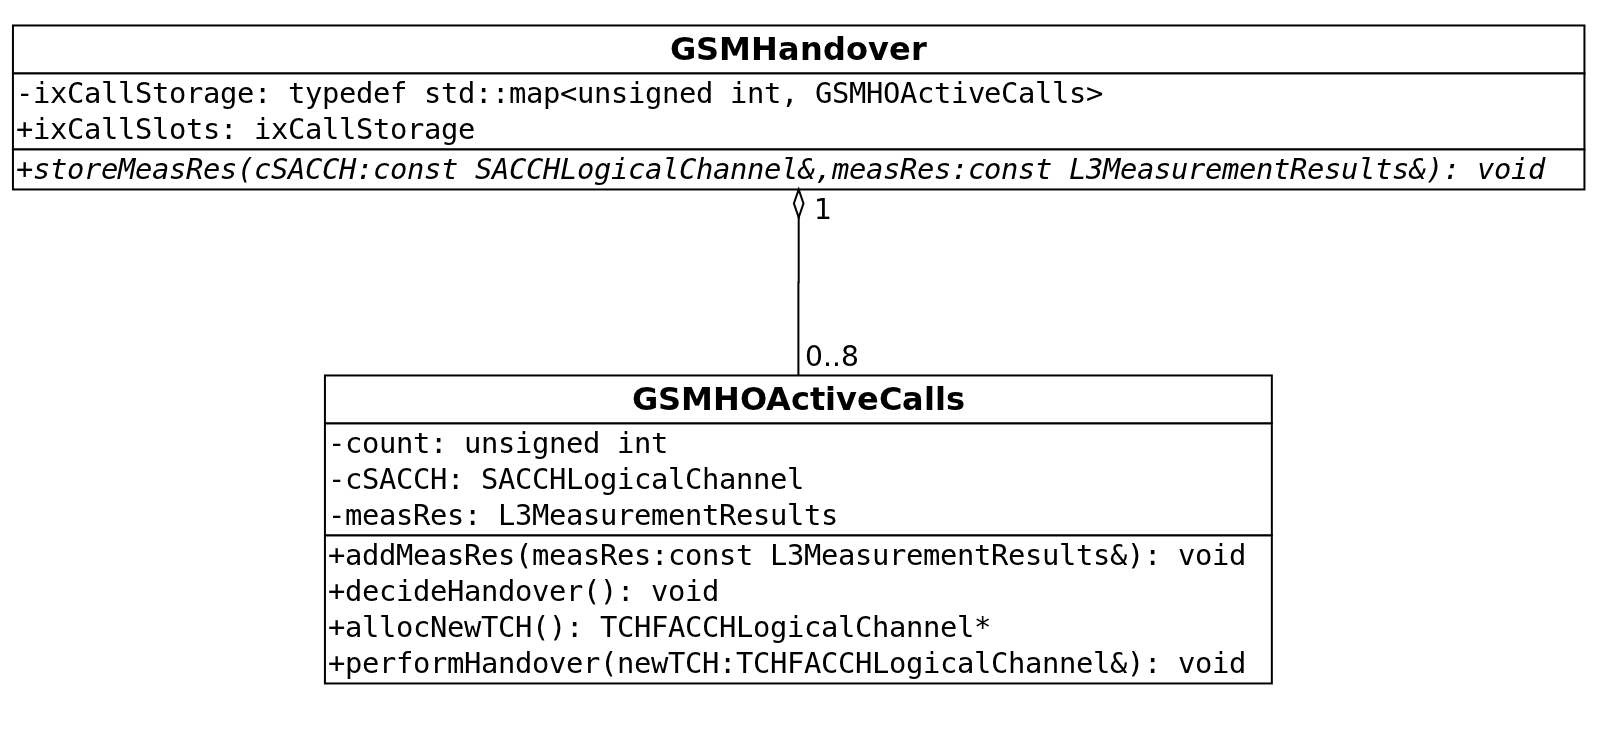
\includegraphics[width=0.8\textwidth]{img/homc}
  \caption{Klassendiagramm Handover-Modul}
  \label{fig:homclass}
\end{figure}

Von der Klasse \lstinline{GSMHandover} wir in der Datei \lstinline{OpenBTS.cpp} des \textit{apps}-Moduls ein globales Objekt instanziiert. Nach dem schreiben der aktuellen Measurement Reports in die SQLite3-Datenbank wird die Methode \lstinline{storeMeasRes()} des \lstinline{GSMHandover}-Objekts aufgerufen. Der Methode werden als Parameter die Referenz auf ein \lstinline{L3MeasurementResults}-Objekt und eine Referenz auf das entsprechende \lstinline{SACCHLogicalChannel}-Objekt übergeben. Mit Hilfe der Frequenz und des Timeslots des \gls{sacch} werden bis zu acht Objekte des Typs \lstinline{GSMHOActiveCalls} in der Map des \lstinline{GSMHandover}-Objekts verwaltet und die neusten Measurement Reports entsprechend zugeordnet.

Die Abarbeitung der restlichen in Abschnitt \ref{sec:handover} beschriebenen Aufgaben erfolgt mit Hilfe der Methoden der Klasse \lstinline{GSMHOActiveCalls}. Die Methode \lstinline{addMeasRes()} überschreibt dabei lediglich das in der Membervariablen gespeicherte Messergebnis. Hier wären zusätzliche Erweiterungen wie die speicherung von beispielsweise bis zu zehn Messergebnissen und die Bildung eines gleitenden Mittelwerts denkbar.

Die Methode \lstinline{decideHandover()} ist für die logische Entscheidungsfindung der Notwendigkeit eines Handover zuständig. In der aktuellen Implementierung prüft die Methode lediglich das vorhandensein der Datei \lstinline{doit} im aktuellen Arbeitsverzeichnis. Auf diese Art kann mit der Eingabe von \lstinline{touch doit} in einer Shell ein Handover manuell für Testzwecke ausgelöst werden. In Zukunft sollte diese Methode die Messergenisse von verscheidenen BTS berücksichtigen und eine logische Entscheidung treffen.

Für den Aufbau eines neuen TCH in einer benachbarten BTS ist eine Kommunikation zwischen den beiden System notwendig. Normalerweise erledigt diese Aufgabe der BSC. Im Fall von OpenBTS diese Kommunikation erst implementiert werden. Diese aufwändige Arbeit konnte im Rahmen der Projektarbeit allerdings nur theoretisch ausgearbeitet werden (siehe Abschnitt \ref{sec:interbts}). Aus diesem Grund wird in der Methode \lstinline{allocNewTCH()} ein TCH innerhalb des aktiven OpenBTS Systems geöffnet.

Der Methode \lstinline{performHandover()} wird als Parameter die Referenz auf den neu allozierten TCH übergeben. Anschließend wird das in Kapitel \ref{sec:swarch} beschriebene Handover-Command erzeugt und über den bestehenden FACCH an die Mobile Station gesendet. Das Umschalten der SIP-Verbindung wäre ein wichtiger Zwischenschritt, der in der aktuellen Implementierung nicht enthalten ist. Neben der Inter BTS Kommunikation, ist diese Aufgabe eine Ansatzpunkt für zukünftige Projektgruppen. Nachdem dem Senden des Handover-Command wir der alte TCH mit Hilfe der entsprechenden GSM-Primitive freigegeben.

Dieser Intra BTS Handover wurde in mehrer Tests erfolgreich durchgeführt und konnte bereits wie in Kapitel \ref{sec:analyse} beschrieben getraced und analysiert werden.

\utsubsection{Inter BTS Kommunikation}{Thomas Waldecker}



\section{Zusammenfassung}




%% Beim Anhang gibt es eine Musterdatei, die 
%% ergänzt werden kann
\appendix
\section{Anhang}
\setcounter{section}{1}


%% einfache Aufz�hlung, kein BibTeX
\subsection{Literaturverzeichnis}
\renewcommand\refname{\vspace*{-2em}}

\begin{thebibliography}{}
\bibitem{bib:grundkursmks} Martin Sauter:
{\it Grundkurs Mobile Kommunikationssysteme},
Vieweg+Teubner Verlag, Wiesbaden 2011

\bibitem{bib:buildopenbsc} Building OpenBSC:
\url{http://openbsc.osmocom.org/trac/wiki/Building_OpenBSC}
Abgerufen am 09.03.2012

\bibitem{bib:ipaccess} ipaccess-config (Konfiguration der nanoBTS):
\url{http://openbsc.osmocom.org/trac/wiki/ipaccess-config}
Abgerufen am 09.03.2012

\bibitem{bib:diagramm:openbts} OpenBTS System Diagramm:
\url{https://wush.net/trac/rangepublic/attachment/wiki/BuildInstallRun/openbts_system_diagram.png},
Abgerufen am 03.03.2012

\bibitem{bib:openbtsmanual} Range Networks Inc.:
{\it OpenBTS P2.8 Users Manual Doc. Rev. 1},
Range Networks Inc. 2011

\bibitem{bib:nokiagammu} AirProbe Wiki - tracelog:
\url{https://svn.berlin.ccc.de/projects/airprobe/wiki/tracelog}, Abgerufen am 09.03.2012

\end{thebibliography}
\leereseite



%% Stichwortverzeichnis ausgeben.
%% falls nicht notwendig, die folgende Zeile loeschen
\printindex

\end{document}
